%!TEX root = ../rapport.tex
%!TEX encoding = UTF-8 Unicode

% Chapitres "Introduction"

% modifié par Francis Valois, Université Laval
% 31/01/2011 - version 1.0 - Création du document


\label{s:experimentation}
\chapter{Laboratoire 2}
\subsection{A)}
L'appareil décrit dans la question est un coupleur directif. Les figures \ref{fig:coupleurdirectif1} et \ref{fig:coupleurdirectif2} représentent le coupleur directif fabriqué par Lab-Volt.
\begin{figure}
\centering
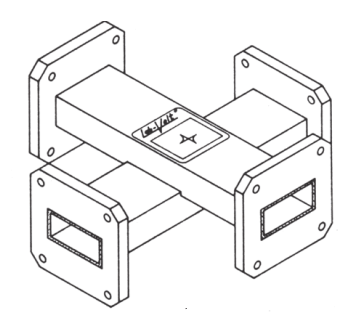
\includegraphics[scale=0.5]{coupleur_directif_1.png}
\caption{Figure montrant une représentation d'un coupleur directif}
\end{figure}
\begin{figure}
\centering
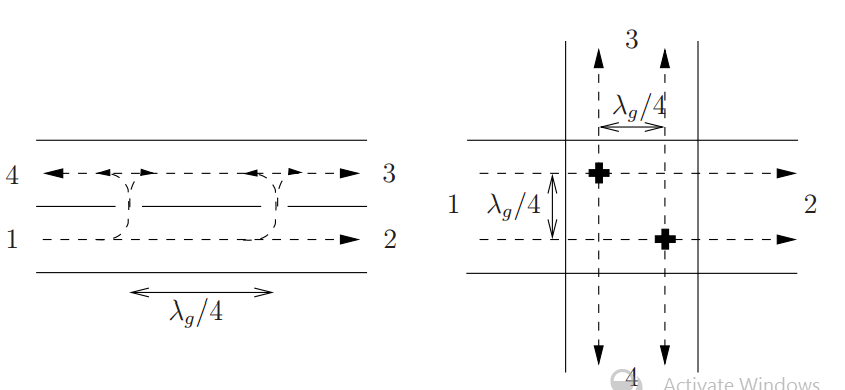
\includegraphics[scale=0.5]{coupleur_directif_2.png}
\caption{Figure montrant une représentation du principe de la propagation des ondes dans un coupleur directif}
\end{figure}

\subsection{B)}
Oui, suivant la courbe v-i de la diode de Gunn, on remarque que pour une tension de polarisation nulle, aucun courant ne circule.

\subsection{C)}
Nous modulons par un signal carré de 1kHz, car l’électronique autour du DC n’est pas facile à réaliser à cause des tensions de polarisation et de décalage qu’on élimine souvent par des condensateurs de découplage ou par des ajustements externes.

\subsection{D)}
En ayant un signal entrant de 2mW et un couplage de 10 dB, nous obtenons un signal C+D de $\frac{2mW}{10} = 200\mu W$. Sachant que le coupleur possède une directivité de 30 dB, nous obtenons les équations suivantes : 

\begin{equation}
	C+D = C+C/1000 = 200\mu W
\end{equation}

En solutionnant, nous trouvons que C = 199.8 $\mu W$ et D = 0.2 $\mu W$.

Si le signal de 2 mW entre dans l'entrée 1, nous obtenons dans l'accès 2 un signal de 1.8 mW, dans l'accès 3, un signal de 199.8 $\mu W$ et dans l'accès 4 un signal de de 0.2 $\mu W$.

\subsection{E}
Pour que l'on se rende compte que la lecture doit être faite dans un calibre de -20 dB au ROS-mètre, on doit soit saturer l'aiguille ou la voir bouger d'une très faible amplitude. Suivant l'un ou l'autre des cas, on décide de simplement changer le calibre de l'appareil afin de profiter d'une déviation supérieure de l'aiguille et ce, sans accoter dans l'une ou l'autre des extrémités. Pour ce faire, il suffit de modifier le calibre vers la plage -20 dB sans modifier le gain intrinsèque ni la fréquence centrale de l'accordeur. 

\subsection{F}
En posant l'hypothèse que le bruit suit une loi de dispersion uniforme et que le signal est contenu dans une bande finie, on suppose que la puissance du bruit sur la puissance du signal augmente avec la largeur de bande. En diminuant la largeur de bande sur l'appareil, on diminue la puissance du bruit sur le signal total. 

\subsection{G)}
Pour produire une oscillation, la diode de Gunn est placée en parallèle avec avec une capacité de 0.6 pF et une résistance négative de l'ordre de -100 $\Omega$. C'est cette résistance qui entretient l'oscillation.

\subsection{H)}
Selon l'échelle Vernier, lorsque le chariot est complètement à droite, la diode se situe à 32.3 mm
\subsection{J}
\subsection{J)}
Une bande longitudinale fait d’un diélectrique à pertes affecte davantage un signal hyperfréquence si elle se situe au centre du guide d’ondes parce que le champ champ électrique est maximal au centre du guide d'onde. 
